% CVPR 2024 Paper Template; see https://github.com/cvpr-org/author-kit

\documentclass[10pt,twocolumn,letterpaper]{article}

%%%%%%%%% PAPER TYPE  - PLEASE UPDATE FOR FINAL VERSION
% \usepackage{cvpr}              % To produce the CAMERA-READY version
\usepackage[review]{cvpr}      % To produce the REVIEW version
% \usepackage[pagenumbers]{cvpr} % To force page numbers, e.g. for an arXiv version

% Import additional packages in the preamble file, before hyperref
%
% --- inline annotations
%
\usepackage[dvipsnames]{xcolor}
\newcommand{\red}[1]{{\color{red}#1}}
\newcommand{\todo}[1]{{\color{red}#1}}
\newcommand{\TODO}[1]{\textbf{\color{red}[TODO: #1]}}
% --- disable by uncommenting  
% \renewcommand{\TODO}[1]{}
% \renewcommand{\todo}[1]{#1}



% It is strongly recommended to use hyperref, especially for the review version.
% hyperref with option pagebackref eases the reviewers' job.
% Please disable hyperref *only* if you encounter grave issues, 
% e.g. with the file validation for the camera-ready version.
%
% If you comment hyperref and then uncomment it, you should delete *.aux before re-running LaTeX.
% (Or just hit 'q' on the first LaTeX run, let it finish, and you should be clear).
\definecolor{cvprblue}{rgb}{0.21,0.49,0.74}
\usepackage[pagebackref,breaklinks,colorlinks,citecolor=cvprblue]{hyperref}
\usepackage{bm}
\usepackage{optidef}
\usepackage[ruled,vlined]{algorithm2e}
\usepackage{multirow}
% \usepackage{subfig}
%%%%%%%%% PAPER ID  - PLEASE UPDATE
\def\paperID{16110} % *** Enter the Paper ID here
\def\confName{CVPR}
\def\confYear{2024}

%%%%%%%%% TITLE - PLEASE UPDATE
\title{Deep Sharpness-Aware Next Best View Selection for Grided View Synthesis}

%%%%%%%%% AUTHORS - PLEASE UPDATE
\author{Anonymous}
% \author{First Author\\
% Institution1\\
% Institution1 address\\
% {\tt\small firstauthor@i1.org}
% % For a paper whose authors are all at the same institution,
% % omit the following lines up until the closing ``}''.
% % Additional authors and addresses can be added with ``\and'',
% % just like the second author.
% % To save space, use either the email address or home page, not both
% \and
% Second Author\\
% Institution2\\
% First line of institution2 address\\
% {\tt\small secondauthor@i2.org}
% }

\begin{document}
\maketitle
\begin{abstract}
Next Best View (NBV) aims at identifying the next most informative sensor position (view) for 3D reconstruction or view synthesis in a 3D scene.
In this paper, we focus on NBV for view synthesis with the emerging representation of implicit voxel grids, which is becoming the game changer with its advantages to recover fine details of the 3D scene while significantly saving training time and training GPU memory footprint.
However, the nature that the latent codes in each voxel cell on the voxel grid are separately and imbalancedly trained induces problem with the existing prediction-based NBV methods where no reasonable information gain prediction can be made across different cells.
To overcome this problem, we present SharpView, an NBV algorithm that first introduces the sharpness of loss space into information gain estimation based on an intuition that the training model has a soft output space around the finely synthesized views.
% This is based on a intuitive observation that the training model has a soft output space around the finely synthesized views, which complies with the continual RGB value shift when the view point of camera is perturbed in the real world.
To estimate sharpness of loss space of a candidate view, we design a pseudo labelling mechanism that incorporates the output of previous trained views and estimate the gradient embedding norm in the last model layer.
We conduct experiments on various view synthesis benchmarks which confirmed that SharpView outperforms the baselines in finding NBV for view synthesis with the representation of implicit voxel grids.
The source code for result reproduction is available at \url{https://github.com/cvpr_16110/SharpView}.
\end{abstract}

\section{Introduction}

% New requirements for NBV for implicit view synthesis
Next Best View (NBV)~\cite{1087372,Biss_NBV,guedon_scone_2022,jin_neu-nbv_2023} aims to iteratively find a shortest and most informative sequence of sensor positions (views) to acquire RGB images in a previous unknown scene to boost efficiency and accuracy of view synthesis of 3D scenes~\cite{sun_direct_2022,li_bnv-fusion_2022,jin_neu-nbv_2023}, which is a fundamental task for downstream applications such as augmented/virtual reality and autonomous driving~\cite{chen_active_2011}.
The existing NBV methods~\cite{shen_stochastic_2021,jin_neu-nbv_2023,ran_neurar_2023} for classic view synthesis typically feature the model representation of a sole multi-layer perception model (MLP) and predicting output uncertainty (e.g., standard deviation) from a view.
% There exists NBV methods~\cite{shen_stochastic_2021,jin_neu-nbv_2023,ran_neurar_2023} for classic view synthesis that typically features the model representation of a sole multi-layer perception model (MLP).
% They typically
% Methods for view synthesis 

However, while the emerging representation of implicit voxel grid for view synthesis (grided view synthesis)~\cite{sun_direct_2022,li_bnv-fusion_2022,zhu_nice-slam_2022} is becoming a game changer of this domain with its advantages to recover fine details of the 3D scene while significantly saving training time and training GPU memory footprint, it is also incurring problems for the existing NBV methods~\cite{shen_stochastic_2021,jin_neu-nbv_2023,ran_neurar_2023} for view synthesis.
Specifically, such representation divides the 3D scene and the training model and map them into pairs of local geometries and local latent codes in grid cells.
And each local latent code is trained to model comparatively a simpler local geometry for fast convergence and only a subset of local latent codes need to be optimized for each view.
% A smaller MLP is responsible to decode local geometries of a view from the local latent codes.
% Each local latent codes only need to model comparatively a simple local geometry for fast convergence and only a subset of local latent codes need to be optimized for each view in view synthesis for minimal GPU memory footprint.
% There exist many NBV methods for explicit 3D scene representation~\cite{guedon_scone_2022} (e.g., point clouds) and implicit 3D scene representation~\cite{shen_stochastic_2021,jin_neu-nbv_2023,ran_neurar_2023} (e.g., multi-layer perception (MLP) model).
% However, the emerging grided 
% This sequence is typically retrieved by iteratively estimating information gain of candidate views and adding the highest one to the sequence.
% While traditional NBV methods process an explicit 3D representation (e.g., point cloud) heuristically or with AI models to find most informative views (e.g., frontiers), the emerging implicit view synthesis methods~\cite{sucar_imap_2021,mildenhall_nerf_2020,li_bnv-fusion_2022,zhu_nice-slam_2022} exploit implicit representation (implicit view synthesis) to achieve finer textural information, scene completion, etc., but also incur difficulty for NBV due to the absence of explicit representation.


% Such training pattern invalidates the existing prediction based NBV methods~\cite{shen_stochastic_2021,jin_neu-nbv_2023,ran_neurar_2023}:
% The existing prediction based NBV methods~\cite{shen_stochastic_2021,jin_neu-nbv_2023,ran_neurar_2023} typically view the model output as a probabilistic distribution (e.g., Gaussian distribution) and train an extra model head for the sole MLP that predicts the uncertainty (e.g., standard deviation) of the model output as the information gain estimation, but they fail to produce reasonable uncertainty prediction in the grided representation.

% Specifically, the representation of implicit voxel grid for view synthesis divides the 3D scene and the training model and map them into pairs of local geometries and local latent codes in grid cells.
% A smaller MLP is responsible to decode local geometries of a view from the local latent codes.
% Each local latent codes only need to model comparatively a simple local geometry for fast convergence and only a subset of local latent codes need to be optimized for each view in view synthesis for minimal GPU memory footprint.
In such case, each voxel cell on the voxel grid are separately and imbalancedly trained and there is often not enough information for a local latent code to model the standard deviation of its output: frequently visited local latent codes will output low uncertainty prediction while those less frequently visited outputs randomly.
We even recorded worse NBV selection performance of the prediction-based NBV methods than the random strategy.

To tackle this problem, we notice an intuition that under small view position and direction perturbation, the observed RGB value of a spot in the 3D scene varies in a continuous way.
It implies that the output space (and loss space) of pixels of the image captured from a finely synthesized view is flat.
Thus the sharpness of the loss space can serve as a hint to find the uncertain views with high information gain, without the need for extra training.
% It implies that for pixels of the image captured from a finely synthesized view, small perturbation in the view position and direction would result

% However, such training pattern invalidates the existing prediction based NBV methods: they typically view the model output as a probabilistic distribution (e.g., Gaussian distribution) and train an extra model head that predicts the uncertainty (e.g., standard deviation) of the model output as the information gain estimation


% Difficulties for uncertainty estimation in implicit NBV
% For implicit representation, a straight-forward estimation of information gain when inputting a candidate view for training is the reduction of uncertainty of model parameters~\cite{tran_bayesian_2019,maddox_simple_2019}, which is, however, reported to be computation expensive and intrusive to the model structure and training process.
% To tackle these problems, prior work~\cite{yan_active_2023,avidan_activenerf_2022,jin_neu-nbv_2023,ran_neurar_2023,shen_stochastic_2021} estimate the uncertainty of model output (e.g., reconstructed 3D scene from a view) as approximation of information gain.
% They typically view the model output as a probabilistic distribution (e.g., Gaussian distribution) and train an extra model head that predicts the uncertainty (e.g., standard deviation) of the model output as the information gain estimation.
% They typically model how much the reconstructed 3D model disagree with the existing training data and implies opportunity for further improvement.
% They train an extra model head to predict the uncertainty (e.g., standard deviation) of the model output and the most uncertain view is selected as NBV.

% However, the cutting-edge grided implicit view synthesis~\cite{li_bnv-fusion_2022,zhu_nice-slam_2022,chabra2020deep,genova2020local} brings challenge to these methods, where they suffer frequent mismatch between estimated uncertainty of model output and actual information gain.
% Specifically, grided implicit view synthesis decomposes the reconstructing 3D scene to a grid of small local geometries and decomposes the training model to a grid of local latent codes, each mapping one small geometry, so that each latent code fits to the reconstructing geometry in real time and also recovers complex local geometries.

% While these methods~\cite{yan_active_2023,avidan_activenerf_2022,jin_neu-nbv_2023,ran_neurar_2023,shen_stochastic_2021} are good at discovering details in candidate views not attended by the training model, the grided implicit view synthesis minimizes such uncertainty with decomposition, and further incurs a new type of uncertainty that they did not consider, uncertainty caused by capacity limit of local latent codes.
% These methods typically assume a simple reconstructing 3D scene and a model large enough to model the whole scene, which do not hold in grided implicit view synthesis, where local latent codes could reach their capacity limit, causing high uncertainty of model output from these latent codes but limited information gain.
% As a result, the NBV selections of these methods often mismatch with the actual improvement of the reconstructed model, causing the lower reconstruction quality reported in our evaluation.
% Also, these methods require inference of the model to estimate uncertainty for each candidate view, which is heavy when the number of candidate views increases for more accurate estimation and even prolonged the whole training process by 1.5$\sim$2 times when estimating 100 candidate views at each NBV selection.

Based on the above observation, we propose SharpView, an NBV algorithm that first introduces the sharpness of loss space into information gain estimation in NBV selection for grided view synthesis.
For estimation of the sharpness of loss space of a view, we generate reasonable pseudo labels (RGB values) by referring the output of the training model from the previously trained views at the same spot as a perturbation for loss computation.
We then back propagate the computed loss against the pseudo labels and compute the sharpness of loss space of a view as the norm of last layer of parameters of the model (the smaller MLP).

In this way, we are able to find the most uncertain views with sharpest loss space, without being influenced by imbalanced training progress of each voxel cell.
We summarize our contributions as follows:
\begin{itemize}
    \item SharpView is the first NBV algorithm that takes sharpness of loss space into consideration for information gain estimation in NBV selection.
    \item We design a pseudo labelling mechanism for new views for sharpness computation.
    \item Sharpness performs best among the baselines in various benchmarks.
\end{itemize}

We discuss the related work in Section~\ref{background}, and introduce our notation, settings and algorithm of SharpView in Section~\ref{methodology}.
We present our experiments in Section~\ref{exp} and then conclude in Section~\ref{conclusion}.
% In the following sections, 




% In this paper, we propose Training-time Uncertainty Estimation for next best View in implicit view synthesis (SharpView).
% Since the local latent codes have limited capacity, instead of predicting output uncertainty, we propose to track the certainty of local latent codes for grided implicit view synthesis.
% Although accurate estimation of uncertainty of model parameters is challenging and computation expensive as stated above, we propose an algorithm Training-Time Certainty Estimation (TTCE) to track how certain the current values of each local latent codes is based on previous training by aggregating and comparing their synaptic dynamics during training, which suffices for NBV selection.
% % In SharpView, we maintain an online estimation of the uncertainty of the latent codes by aggregating their synaptic dynamics during training.
% Leveraging the knowledge about the 3D correspondence of each local latent codes, we are able to distinguish the local latent codes within the camera frustum of a view and render their estimated certainty to an image for each candidate view as information gain estimation, without incurring any extra training or inference computation burden.
% As a result, SharpView is suitable for edge devices with limited computation resources such as robots where NBV for view synthesis is typically deployed.
% As the grided latent codes each have their 3D correspondence in the 3D scene, we estimate the uncertainty of latent codes visited by candidate views (lying within their camera frustums) for NBV selection.
% In this way, SharpView gets more accurate estimation of possible information gain of candidate views for implicit view synthesis, boosting efficiency and accuracy of implicit view synthesis.
% Also, these advantages are achieved without the need of training any extra model or incurring any extra inference computation burden, making SharpView suitable for edge devices with limited computation resources such as robots where NBV for view synthesis is typically deployed.


% Specifically, implicit view synthesis encodes 3D scene information from a sequence of views (images captured at corresponding sensor positions) to a grided latent space, with a decoder able to extract 3D scene from the latent codes.
% The latent codes are periodically optimized, minimizing the discrepancies between decoded 3D scene and ground-true view measurements to extract finer geometry and textural information.

% To estimate information gain of candidate views in implicit view synthesis, prior work typically treat decoded 3D scene as a Gaussian distribution.
% They either online or offline train an extra model head on the decoder to predict the uncertainty (e.g., standard deviation) of decoded 3D scene from a view and the most uncertain view is selected as NBV.
% However, such methods require inference of the model to predict uncertainty for each candidate view, which is heavy when the number of candidate views is increased for more accurate estimation, especially for edge devices such as robots exploring large scenes.
% % Worse, the predicted uncertainty itself suffers uncertainty: the uncertainty intuitively represents the possibility of decoded 3D scene to differ from the ground truth, and such uncertainty estimation gets more accurate only when more reference views are input, making their choice of NBV often mismatch with the most informative.
% Worse, sampling views of high estimated uncertainty of the decoded 3D scene does not necessarily lead to high improvement of it, since the capacity of latent codes has its limit.
% Thus prediction-based NBV tend to be stuck around certain spots of high uncertainty, while the information gain is limited.

% Specifically, implicit view synthesis encodes 3D scene information from views (images captured at corresponding sensor positions) to a grided latent space, with a decoder able to extract 3D scene from the latent space given 3D coordinate query.
% The latent space is periodically optimized under the supervision of captured views to extract geometry and textural information.
% The key reason for the difficulty of prediction based methods is that the uncertainty of decoded 3D scene at a coordinate intuitively represents its possibility to differ from the ground truth, and such uncertainty estimation gets more accurate only when more reference views are input, which means less uncertain. 
% To alleviate these problems, we observe that the possible information gain of a new view is fundamentally related to how much the underlying latent codes can be changed by training with this view being input, or more precisely the uncertainty of the latent codes after being trained with existing views.
% Inspired by studies of continual learning, if we treat training the latent codes based on a newly captured view (together with previously captured views) as a new task, the uncertainty of the latent codes can be represented as how much the latent codes were consolidated by previous training, computed based on the synaptic dynamics (gradient and parameter update records) during training.

% As the grided latent codes each have their 3D correspondence in the 3D scene, estimating the uncertainty of latent codes visited by candidate views can provide hints for NBV selection in implicit 3D rendering.

% In this paper, we propose Training-time latent code Uncertainty Estimation for next best View in implicit view synthesis (SharpView).
% In SharpView, we maintain an online estimation of the uncertainty of the latent codes by aggregating their synaptic dynamics during training.
% As the grided latent codes each have their 3D correspondence in the 3D scene, we estimate the uncertainty of latent codes visited by candidate views (lying within their camera frustums) for NBV selection.
% In this way, SharpView gets more accurate estimation of possible information gain of candidate views for implicit view synthesis, boosting efficiency and accuracy of implicit view synthesis.
% Also, these advantages are achieved without the need of training any extra model or incurring any extra inference computation burden, making SharpView suitable for edge devices with limited computation resources such as robots where NBV for view synthesis is typically deployed.

% The main contributions of this paper are as follows:
% \begin{itemize}
%     \item We introduce an efficient uncertainty estimation algorithm (TTCE) for the emerging representation of grided local latent codes that tracks the certainty of local latent codes purely from synaptic dynamics collected during training. Compared with prior work, our proposed algorithm directly operates on latent codes and incurs little computation burden, making it suitable for edge devices where NBV is typically deployed.
%     \item We propose a new next-best-view system (SharpView) for the emerging grided implicit view synthesis. By directly rendering the estimated certainty of grided latent codes, we avoid the interference of capacity limit of local latent codes and get more accurate estimation of possible information gain of candidate views, boosting the efficiency and accuracy of implicit view synthesis.
%     \item Experiments on various complex 3D objects and large scale indoor scenes show that SharpView improved the quality of the reconstructed 3D model over the baselines, while only introducing a negligible (about 10\%) extra computation time. The source code to reproduce our results is publicly released at \url{https://github.com/aaai_5846_paper/SharpView}.
% \end{itemize}


\section{Background\label{background}}
\subsection{Neural Implicit Representations}
Neural implicit representation~\cite{mildenhall_nerf_2020,sucar_imap_2021,li_bnv-fusion_2022,zhu_nice-slam_2022,jin_neu-nbv_2023} is a emerging mapping representation demonstrating promising results for object geometry reconstruction, scene completion, novel view synthesis and also generative modelling.
They typically feature a Neural Radiance Field (NeRF)~\cite{mildenhall_nerf_2020} structure that learns a density and radiance field supervised by 2D views (camera position \& orientation and the images captured) with an MLP model.
iMAP~\cite{sucar_imap_2021} uses a single MLP neural model as the underlying 3D scene representation and with a comparatively simple implicit representation and efficient rendering pipeline, iMAP achieves near real-time performance in training.

However, recent researches~\cite{chabra2020deep,9156855,genova2020local,li_bnv-fusion_2022,zhu_nice-slam_2022} report a single MLP representation is not scalable due to limited capacity and tends to ignore complex details.
They propose to decompose the whole 3D scene to grided local scenes and train local implicit representations to map the local geometry in each local scene, 
which improves the level of detail in reconstruction because each local implicit representation only needs to map a local region rather than the geometry of a whole scene.
Organizing the local implicit representations as a grid, we can easily find the 3D correspondence between the local implicit representations and the 3D scene, which is the basis of our proposed method.

\subsection{Grided Implicit Rendering}
Along the decomposition of the implicit representation to grided local implicit representations, some~\cite{li_bnv-fusion_2022,zhu_nice-slam_2022} also decompose the training pipeline to effectively leverage prior knowledge of local geometries embedded in MLP.
Specifically, they~\cite{li_bnv-fusion_2022,zhu_nice-slam_2022} separate the MLP model to an AutoEncoder-like network that consist of an encoder, grided latent codes and a decoder, with the encoder and the decoder pretrained over various scenes to extract generalizable knowledge of 3D reconstruction.
Because they only need to optimize the local latent codes, they manage to reconstruct complex geometry of 3D scenes in a view with several training iterations, retaining real-time performance as imap~\cite{sucar_imap_2021}.
Among these work, we select BNV-Fusion~\cite{li_bnv-fusion_2022} as our major research target, which takes depth images and camera poses as input and achieves high quality shape reconstruction of complex 3D scene.

\subsection{Next Best View}
Traditional NBV~\cite{Biss_NBV,guedon_scone_2022,1087372} typically aims to find a shortest sequence of views from a set of candidate views that optimize the coverage of a previously unknown area.
Given the existing partial explicit map (e.g., point cloud), they either heuristically find frontiers of the map, or predict views with AI models that optimize coverage.
With the emerging implicit 3D reconstruction being able to reconstruct finer details of the complex 3D scene, optimizing accuracy is also an emerging requirement for NBV~\cite{avidan_activenerf_2022,jin_neu-nbv_2023,ran_neurar_2023,shen_stochastic_2021}, where the most valued information gain is the improvement of the quality of the reconstructed 3D model.

\subsection{Uncertainty Estimation}
The information gain from training data for a training model can be directly modeled as the uncertainty reduction of model parameters, and such uncertainty estimation is a long-standing problem~\cite{ABDAR2021243,gal2016dropout,lakshminarayanan2017simple,maddox_simple_2019,tran_bayesian_2019,bissiri_general_2016} for machine learning.
A classic framework for uncertainty estimation is the Bayesian Learning framework that estimates the posterior distribution of the model given the existing training data.
% The posterior distribution can reflect the uncertainty of the model output during inference.
However, such approaches typically require multiple model evaluations which are computationally expensive, and require significant modifications over network architectures and training procedures~\cite{shen_stochastic_2021,tran_bayesian_2019}.

Recent work focusing on the NeRF structure approximate the uncertainty of model parameters with the posterior distribution of the output density and radiance (uncertainty of the model output)~\cite{shen_stochastic_2021,avidan_activenerf_2022,ran_neurar_2023,jin_neu-nbv_2023}.
They typically follow the pattern of generalization of standard NeRF~\cite{shen_stochastic_2021} that learns a probability distribution over all the possible radiance fields modeling the scene, 
where an extra model head is trained to estimate the variance of the radiance fields under the supervision of existing views.

% In the case of a sole MLP modelling the whole 3D scene, 

% However, when facing the representation of implicit voxel grid, due to the nature that each voxel cell on the voxel grid are separately and imbalancedly trained

% Intuitively, the standard deviation of distribution of model output stems from the model not attending to high-frequency details.
% However, the grided implicit 3D reconstruction~\cite{li_bnv-fusion_2022,zhu_nice-slam_2022} on the one hand minimizes such uncertainty by decomposition, on the other hand incurs an extra source of uncertainty caused by the capacity limit of local latent codes, which severely disturbs the NBV selection of the prior methods by incurring high uncertainty of model output and limited information gain from certain views.
% As a result, these methods tend to be stuck at certain spots where the corresponding local latent codes reach their capacity limit, causing inefficiency.

% Using a finer-grained (denser) grid of latent codes seems to be a simple remedy, which avoids the local latent codes to reach their modeling capacity, but this remedy results in a much larger model size and GPU memory consumption and also, it is reported~\cite{li_bnv-fusion_2022,zhu_nice-slam_2022} a too fine-grained grid of latent codes results in not enough training data input within each local region (number of rays casting to each local latent codes will be reduced) for training the local embedding, causing holes in the reconstructed model.
% In a word, the uncertainty caused by the capacity limit of local latent codes would be a common problem in grided implicit 3D reconstruction.


% However, a major difficulty of these methods is that uncertainty of the model output often mismatches with uncertainty of the local latent codes in implicit 3D reconstruction.
% Intuitively, uncertainty in implicit 3D reconstruction comes from three sources: uncertainty caused by limited capacity of the model, uncertainty caused by model not attending to high-frequency details that can be optimized by further training and sampling, noises.
% The posterior distribution of the output is good at discovering the second type of uncertainty by 


% \subsection{Continual Learning}
% categories  memory, multi-task, regularization,
\subsection{Connection to Other Sharpness Methods}
In the domain of active learning, there exists other methods~
\cite{keskar_large-batch_2017,ash_deep_2020,jiang_fantastic_2019,kim_saal_2023} that also inspect the flatness of loss space and use gradients as an indicator of its sharpness.
To the best of our knowledge, they~\cite{keskar_large-batch_2017,ash_deep_2020,jiang_fantastic_2019,kim_saal_2023} are focused on classification problems where the model output is the activated by a softmax function and the pseudo labelling policy is simply selecting the value with highest probability in the output, which cannot work with implicit rendering pipeline where rgb values are directly output .
We are the first work to connect loss space sharpness with implicit rendering pipeline by introducing the pseudo labelling policy based on the intuition of continuity of rgb values around a small region of viewpoints.

\subsection{Grided View Synthesis}
Here we discuss the notation of grided view synthesis in details.
Assume that we equally divide the 3D scene of interest into $M$ cells under certain resolution and the
implicit voxel grid for view synthesis can be represented as pairs of 3D coordinates of local geometries and local latent codes modelling the local geometry: $G=\{(x_i,\theta_i)\}_{i=1}^M$.
Given a step on a ray $r=(x,d)$ where $x$ is a coordinate in the 3D scene and the $d$ is the viewing direction, we query the pairs for the closest distance $\theta_j = Q(G,r)$ and then use MLP models to decode the density $\sigma$ and view-direction-dependent color $c$ from the corresponding local latent codes: $\sigma,c=MLP(\theta_j, d)$.

To render the color $C(r)$ of a pixel on an image from a view, we cast a ray with $K$ steps, $\bm{r}=\{r_i\}_{i=1}^K$ from the center of the camera through the pixel and query the implicit voxel grid for density and rgb values at each step $\{\sigma_i, c_i\}_{i=1}^K$.
Finally, the queried results are accumulated to compute $C(r)$.
\begin{subequations}
    \begin{align}
        \label{accu}
        C(\bm{r}) &= \sum_{i=1}^{K}T_i \alpha_i c_i \\
        \alpha_i &= 1 - exp(-\sigma_i \delta_i) \\
        T_i &= \prod_{j=1}^{i-1} (1-\alpha_j)
    \end{align}
\end{subequations}
where $\alpha_i$ is the probability of termination of ray at step $i$, $T_i$ is the accumulated transmittance and $\delta_i$ is the distance between consecutive steps.
% \begin{equation}
%     C(r)=\sum_{i=1}^{K}T_i \alpha_i c_i
% \end{equation}
We gather the rgb value of each pixel on the image from a view and forms the predicted image $I$ from view $v$ and the loss is calculated against the groundtruth image $\hat{I}$ with mean square error $l_{mse}(I, \hat{I})$.
\section{Methodology\label{methodology}}
% \begin{figure*}
%     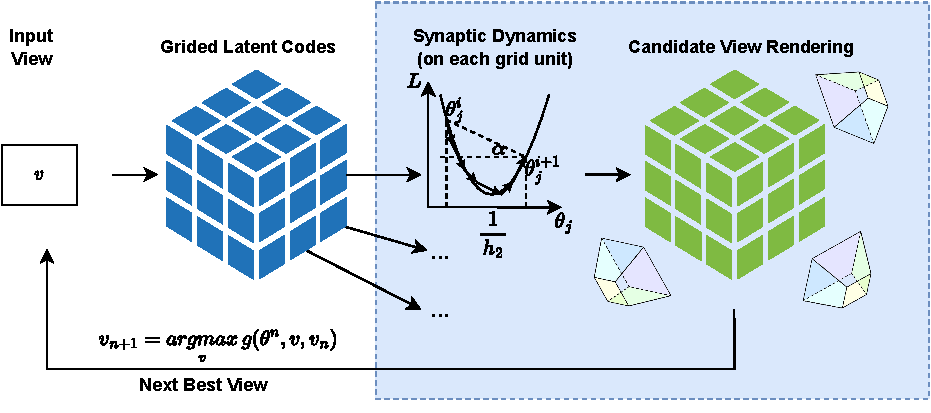
\includegraphics{overview.pdf}
%     \caption{Overview of the loss space sharpness estimation pipeline of SharpView. The left blue grid is the grid of local latent codes of grided view synthesis. The right green grid is the corresponding data grid to store the certainty estimation of each local latent codes and we directly estimate the information gain of each candidate view by directly rendering their certainty estimation in the camera frustum.}
%     \label{overview}
% \end{figure*}
Given a set of $N$ views $V=\{v_i\}_{i=1}^N$ discretized on a sphere, assume the above grided view synthesis pipeline has been trained by a subset $S\subset V$ and their corresponding groundtruth images, and the candidate views for NBV selection is $U=\frac{V}{S}$.
We approximate the information gain of a view with the value of loss function of the grided view synthesis pipeline.
To solve the NBV problem, we aim to find a view that maximize the loss between rendered image from the view and the corresponding groundtruth image, which typically complies with the sharpest loss space around the view.

\subsection{Pseudo Ray Labelling}

\begin{algorithm}[htb]
    \caption{Pseudo Ray Labelling}
    \label{alg:ray}
    \KwIn{A ray: $\bm{r}$; Set of trained views: $S$; implicit voxel grid: $G$}
    \KwOut{Pseudo accumulated rgb value of $\bm{r}$: $\hat{C}(\bm{r})$}
    \BlankLine
    
    Compute the dominant step $r^d$ along $r$;
    
    Compute the closest view $v'\in S$ from $r^d$;
    
    Cast ray $\bm{r}'$ from $v'$ to $r^d$;
    
    Render pseudo rgb value $\hat{C}(\bm{r})$ of $\bm{r}'$ from $G$.
\end{algorithm}
To compute a reasonable pseudo label for loss calculation to estimate sharpness of loss space, we use views in $S$ as references assuming that the implicit voxel grid has already fully learned knowledge from their corresponding images.
Assume we are estimating loss space sharpness of a candidate view $v$ and we are casting a ray $\bm{r}$ with $K$ steps to predict the rgb value of a pixel on the predicted image from view $v$.

In view of the continuity of rgb value when the viewing direction is slightly perturbed, a reasonable pseudo label for ray $\bm{r}$ would be the rgb value predicted from the closest trained view, which is also the most certain value that can be predicted from the grid.
As shown in Algorithm~\ref{alg:ray}, to compute the closest trained view, we first find a dominant step $r^d$ along $\bm{r}$:
\begin{equation}
    \begin{aligned}
        r^d &= r_k \\
        k & =\mathop{\arg\max}\limits_{0<i \leq K} T_i \alpha_i
    \end{aligned}
\end{equation}
$\alpha_i$ and $T_i$ are the probability of termination of ray at step $i$ and the accumulated transmittance from Equation~\ref{accu} when rendering accumulated rgb value along $\bm{r}$.
We are treating the term $T_i \alpha_i$ as weights of each step and the one with largest weight is the dominant one.

Then we cast rays from all trained views to the coordinate $x^d$ determined by $r^d$ and the ray with smallest intersection angle with $r^d$ is selected as the reference ray, and we render the rgb value $\hat{C}(\bm{r})$ of this reference ray as the pseudo label for $\bm{r}$.

\subsection{Sharpness Estimation}
The procedure of loss space sharpness estimation for a view $v$ in shown in Algorithm~\ref{alg:sharpness}.
Gathering pseudo label of each ray through each pixel on the predicted image $I$ from view $v$ we will get a pseudo image $\hat{I}$. 
After computing mean square error loss between $I$ and $\hat{I}$ and back propagating the loss, we use the norm of gradients of weights from the last layer of decoder MLP as an estimation of sharpness.
After estimating the sharpness among all candidate views in $U$, the one with highest sharpness value is selected as the next best view $v_n$.
We then acquire its groundtruth image, append to the training set $S$ and remove it from the candidate set $U$.

\begin{algorithm}[htb]
\caption{Loss Space Sharpness Estimation}
\label{alg:sharpness}
\KwIn{A candidate view: $v$; Set of trained views: $S$; implicit voxel grid: $G$; MLP decoder: $M$}
\KwOut{Sharpness of loss space around $v$: $s$}
\BlankLine
Render predicted image $I$ of $v$ with $G$ and $M$;

$\hat{I}$ = copy($I$);

\For{pixel $\in \hat{I}$}{

    Cast ray $\bm{r}$ from $v$ to pixel;

    $\hat{C}(\bm{r})$ = PseudoRayLabelling($\bm{r}$, $S$, $G$);

    Replace pixel value on $\hat{I}$ with $\hat{C}(\bm{r})$;
}

Back propagate $g_I = \frac{\partial}{\partial M_{out}} l_{mse}(I, \hat{I})$, where $M_{out}$ is the weight of the final layer;

$s$ = $\Vert g_I \Vert_2$.
\end{algorithm}
% The subtlety behind this procedure is that 

% \subsection{Next Best View}
% Given a dataset of N views discretized on a sphere $\bm{v}=\{v_i\}_{i=1}^N$, an acquisition function retrieves the groundtruth RGB image $I$ captured from a view and adds it to the training view set $S$ for training the above grided view synthesis pipeline.
% The candidate view set not yet being trained is defined as $U=\frac{\bm{v}}{\{v|v\in S\}}$.

% To solve 


\section{Experiments\label{exp}}
\subsection{Evaluation Setup}
\subsubsection*{TestBed} We evaluated SharpView on a PC equipped with Nvidia 2080Ti 11GB GPU, Intel i5-12400 CPU and 32GB RAM. 

\subsubsection*{Baselines} We compare SharpView (referred to as Sharp.) against three baselines: random (referred to as Rand.), maximal distance (referred to ass MDist.) and prediction-based NBV (referred to as Pred.).
Rand. is a pure randomized strategy.
MDist. maximizes the distance between selected view to the view from the training dataset.
Pred. is a prediction-based method that trains an extra head on the MLP decoder of the grided view synthesis pipeline
following the patterns of loss functions commonly used in these methods~\cite{shen_stochastic_2021,jin_neu-nbv_2023,ran_neurar_2023,avidan_activenerf_2022}: 
\begin{equation}
    L = \frac{1}{R} \sum_{r=0}^R  \big ( \log \sigma_r + \frac{(c_r-\hat{c}_r)^2}{\sigma_r^2} \big )
    \label{uncertainty}
\end{equation}
where $R$ is the number of pixels in an input image, $\sigma_r$ is the standard deviation prediction from the extra model head, $c_r$ is the predicted rgb value, and $\hat{c}$ is the groundtruth rgb measurement.

\subsubsection*{Workload}
We choose DirectGO~\cite{sun_direct_2022} as the grided view synthesis pipeline for our evaluation, which features a implicit voxel grid representation of the 3D scene and short convergence time within minutes, compared with the convergence time of days using the non-grided counterparts.
It also achieves comparable resulting view synthesis accuracy.
We follow DirectGO to use PSNR, SSIM~\cite{1284395}, and LPIPS~\cite{8578166} as the metrics to compare the view synthesis accuracy among SharpView and the baselines.

\subsubsection*{Datasets}
We evaluate our approach on three different datasets. We configure the datasets mainly following the default setup of DirectGO~\cite{sun_direct_2022}. Synthetic-NeRF contains eight objects with realistic images synthesized by NeRF. Synthetic-NSVF contains another eight objects synthesized by NSVF. We follow the setup of these two datasets and set the image resolution to 800 $\times$ 800 pixels and set 100 views for training and NBV selection and 200 views for testing for each scene.
TanksAndTemples is a real-world dataset captured from large real-world 3D scenes with  1920 $\times$ 1080 image resolution. We set one-eighth of the images testing and the rest for training and NBV selection.

\subsubsection*{NBV Configuration}
We initialize the NBV procedure by training the grided view synthesis pipeline with a initial training dataset sized six views.
And the NBV procedure ceases after acquiring ten new views from the training dataset.
The six views are selected by randomly selecting the first view and then append the rest views with the same policy with MDist., so that all surfaces of the 3D scene are more likely to be covered at the initial stage.
After a view is appended to the training set, we retrain the grided view synthesis pipeline to avoid overfitting to the previous views in the training set and compute new NBV information gain estimation.
In the training procedure, we scale the default configuration of number of training iterations and learning rate decay from DirectGO~\cite{sun_direct_2022} by the ratio between the length of training set and the whole training dataset.
At the end of the NBV procedure, the view synthesis accuracy results are calculated and
we present below the results averaged over repeating the evaluation with three different seeds.
% The results below are averaged on the results evaluated with three different seeds.



\subsection{Quantitative Comparison}
We first qualitatively compare the view synthesis accuracy results under different NBV methods.
With the knowledge of loss space sharpness of each candidate views, SharpView managed to select views with more information gain from the candidate views as the NBV, and constantly outperformed the baselines in terms of PSNR, SSIM and LPIPS as shown in Table~\ref{nsvf}, ~\ref{nerf} and~\ref{tank}.

Note that while the results of Rand. and MDist. are comparable since they are both naive methods without any information gain estimation, Pred. constantly performed the worst, which means that Pred. tended to select views with less information gain in the grided view synthesis settings.
The possible reason for this phenomenon is two-fold.
First, the extra term and factor introduced in their loss function as in Equation~\ref{uncertainty} in additional to the mean square error may decrease the magnitude of the computed loss value and thus slow down convergence.
Second, the local latent codes in different cells are separately and imbalancedly trained, which means the supervision of certain cells can be weak, especially the less frequently visited and thus uncertain cells.
This results in that the frequently visited cells output low uncertainty (standard deviation of its rgb output $\sigma$) and less frequently visited cells output uncertainty of comparatively random values, severely interfering their NBV selection.



\begin{table*}[h!]
    \centering
    \caption{Results on Synthetic-NSVF. }
    \begin{tabular}{|c|c|c|c|c|c|c|c|c|c|}
        \hline
        \multirow{2}{*}{Methods} & \multicolumn{3}{c|}{Palace} &  \multicolumn{3}{c|}{Robot} &  \multicolumn{3}{c|}{Spaceship} \\ \cline{2-10}
         & PSNR$\uparrow$ & SSIM $\uparrow$& LPIPS $\downarrow$ & PSNR$\uparrow$ & SSIM $\uparrow$& LPIPS $\downarrow$& PSNR $\uparrow$& SSIM $\uparrow$& LPIPS $\downarrow$

         \\ \hline Rand.  & 27.841 & 0.884 & 0.084 & 25.777 & 0.949 & 0.047 & 26.181 & 0.944 & 0.05
         \\ \hline MDist.  & 27.56 & 0.879 & 0.082 & 25.357 & 0.946 & 0.049 & 25.805 & 0.942 & 0.05
         \\ \hline Pred.  & 26.111 & 0.849 & 0.118 & 23.454 & 0.929 & 0.070 & 24.049 & 0.928 & 0.073
         \\ \hline Sharp.  & $\bm{28.768}$ & $\bm{0.897}$ & $\bm{0.069}$ & $\bm{27.653}$ & $\bm{0.963}$ & $\bm{0.025}$ & $\bm{26.561}$ & $\bm{0.948}$ & $\bm{0.047}$
         \\ \hline
    \end{tabular}
    \label{nsvf}
\end{table*}

\begin{table*}[h!]
    \centering
    \caption{Results on Synthetic-NeRF. }
    \begin{tabular}{|c|c|c|c|c|c|c|c|c|c|}
        \hline
        \multirow{2}{*}{Methods} & \multicolumn{3}{c|}{chair} &  \multicolumn{3}{c|}{lego} &  \multicolumn{3}{c|}{ship} \\ \cline{2-10}
         & PSNR$\uparrow$ & SSIM $\uparrow$& LPIPS $\downarrow$ & PSNR$\uparrow$ & SSIM $\uparrow$& LPIPS $\downarrow$& PSNR $\uparrow$& SSIM $\uparrow$& LPIPS $\downarrow$

         \\ \hline Rand.  & 26.03 & 0.916 & 0.082 & 25.889 & 0.904 & 0.062 & 23.871 & 0.797 & 0.192
         \\ \hline MDist.  & 27.034 & 0.928 & 0.07 & 26.392 & 0.911 & 0.056 & 24.609 & 0.798 & 0.184
         \\ \hline Pred.  & 23.224 & 0.871 & 0.129 & 22.521 & 0.842 & 0.117 & 22.744 & 0.747 & 0.227
         \\ \hline Sharp.  & $\bm{28.573}$ & $\bm{0.936}$ & $\bm{0.049}$ & $\bm{27.133}$ & $\bm{0.919}$ & $\bm{0.047}$ & $\bm{25.116}$ & $\bm{0.805}$ & $\bm{0.171}$
         \\ \hline
    \end{tabular}
    \label{nerf}
\end{table*}


\begin{table}[h!]
    \centering
    \caption{Results on TanksAndTemple (Averaged across different scenes). }
    \begin{tabular}{|c|c|c|c|}
        \hline
        Methods & PSNR$\uparrow$ & SSIM $\uparrow$& LPIPS $\downarrow$ 

         \\ \hline Rand.  & 21.369 & 0.871 & 0.210
         \\ \hline MDist.  & 21.188 & 0.867 & 0.217
         \\ \hline Pred.  & 17.437 & 0.837 & 0.264
         \\ \hline Sharp.  & $\bm{22.674}$ & $\bm{0.879}$ & $\bm{0.200}$
         \\ \hline
    \end{tabular}
    \label{tank}
\end{table}

\subsection{Qualitative Comparison}
Here we present some details of the tested view synthesis results after the NBV procedure of each method for qualitative comparison, which shows that synthesized views with SharpView recovered finer details of the 3D scenes.


\begin{figure*}[ht!]
    \centering
      \begin{subfigure}{0.19\textwidth}
        \centering   
        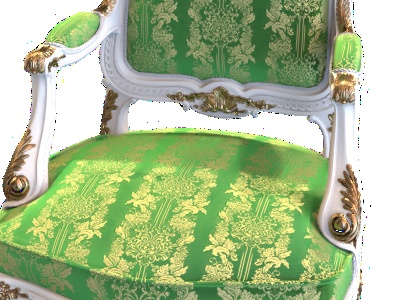
\includegraphics[width=\linewidth]{figs/gt_chair.jpg}
          \caption{groundtruth}
          \label{fig:sub1}
      \end{subfigure}   %      \hfill  % 这个\hfill指令为插入弹性长度的空白,看情况选择加不加。
      \begin{subfigure}{0.19\textwidth}
        \centering   
        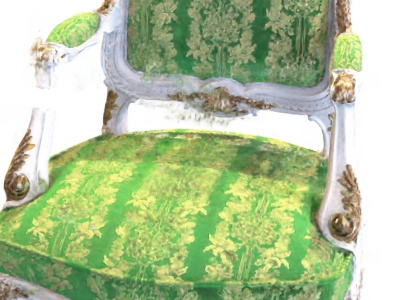
\includegraphics[width=\linewidth]{figs/random_chair.jpg}
          \caption{Rand.}
          \label{fig:sub2}
      \end{subfigure}
      \begin{subfigure}{0.19\textwidth}
        \centering   
        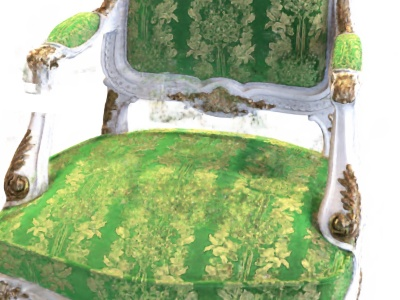
\includegraphics[width=\linewidth]{figs/max_dist_chair.jpg}
          \caption{MDist.}
          \label{fig:sub2}
      \end{subfigure}
      \begin{subfigure}{0.19\textwidth}
        \centering   
        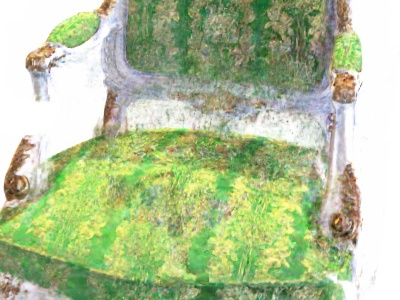
\includegraphics[width=\linewidth]{figs/uncertainty_chair.jpg}
          \caption{Pred.}
          \label{fig:sub2}
      \end{subfigure}
      \begin{subfigure}{0.19\textwidth}
        \centering   
        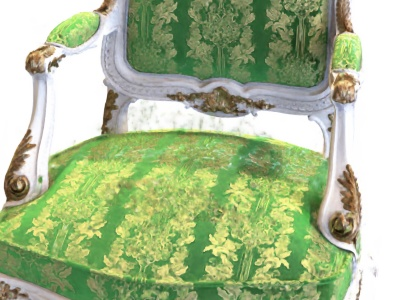
\includegraphics[width=\linewidth]{figs/sharpness_chair.jpg}
          \caption{Sharp.}
          \label{fig:sub2}
      \end{subfigure}
  \caption{
  \label{fig:total}
  Qualitative Comparison on Synthesis Nerf chair.
  }
\end{figure*}


\begin{figure*}[ht!]
    \centering
      \begin{subfigure}{0.19\textwidth}
        \centering   
        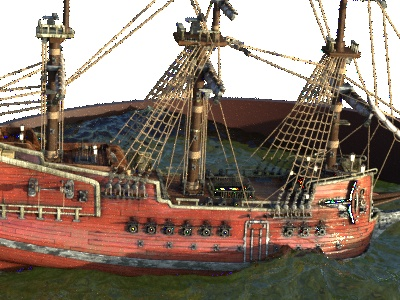
\includegraphics[width=\linewidth]{figs/gt_ship.jpg}
          \caption{groundtruth}
          \label{fig:sub1}
      \end{subfigure}   %      \hfill  % 这个\hfill指令为插入弹性长度的空白,看情况选择加不加。
      \begin{subfigure}{0.19\textwidth}
        \centering   
        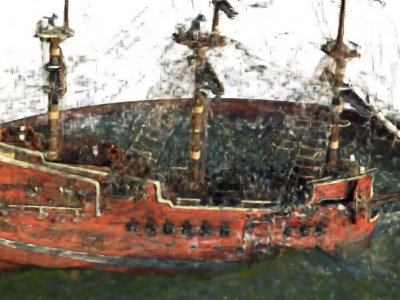
\includegraphics[width=\linewidth]{figs/random_ship.jpg}
          \caption{Rand.}
          \label{fig:sub2}
      \end{subfigure}
      \begin{subfigure}{0.19\textwidth}
        \centering   
        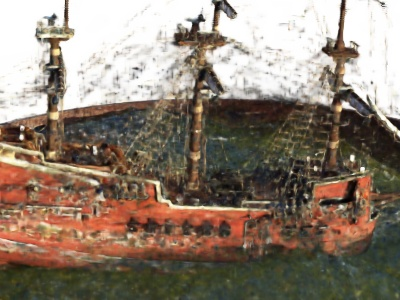
\includegraphics[width=\linewidth]{figs/max_dist_ship.jpg}
          \caption{MDist.}
          \label{fig:sub2}
      \end{subfigure}
      \begin{subfigure}{0.19\textwidth}
        \centering   
        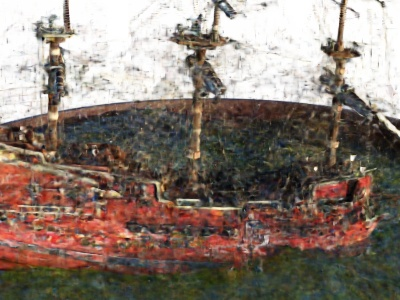
\includegraphics[width=\linewidth]{figs/uncertainty_ship.jpg}
          \caption{Pred.}
          \label{fig:sub2}
      \end{subfigure}
      \begin{subfigure}{0.19\textwidth}
        \centering   
        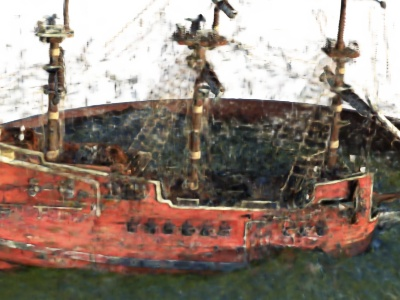
\includegraphics[width=\linewidth]{figs/sharpness_ship.jpg}
          \caption{Sharp.}
          \label{fig:sub2}
      \end{subfigure}
  \caption{
  \label{fig:total}
  Qualitative Comparison on Synthesis Nerf ship.
  }
\end{figure*}

\subsection{Discussion and Limitation}
Due to limited time budget, we did not make it to broadly and extensively evaluate SharpView and we are taking it as the future work.
Although we are motivated by the problems induced by grided view synthesis, the resulting algorithm and pipeline does not rely on the architecture or design of grided view synthesis, and we are curious about whether similar advantages can be achieved on other view synthesis architecture or even other domain of implicit rendering such as 3D reconstruction, which is also regarded as our future work.
\section{Conclusion\label{conclusion}}
While the cutting-edge grided view synthesis boost the state-of-the-art performance of view synthesis, it incurs difficulty for NBV selection since latent codes in the grid are imbalancedly trained.
In this paper, we present SharpView, the first NBV algorithm for grided view synthesis that incorporates loss space sharpness estimation into information gain estimation for NBV selection.
By simply leveraging pseudo ray labelling, we estimate the sharpness of loss space of the current training model at candidate views by calculating the gradients of parameters of the last layer of the view synthesis pipeline, without the need to train or infer extra information from the latent codes, so that more accurate information gain estimation can be achieved.
% In this paper, we present Training-time Uncertainty Estimation for next best View in implicit 3D reconstruction (SharpView).
% SharpView estimates certainty of local latent codes and leverages the 3D corresponding between local latent codes and the local geometries in the 3D scene to estimate certainty to render and estimate the potential information gain from candidate views to get an more accurate modelling of possible model improvement.
{
    \small
    \bibliographystyle{ieeenat_fullname}
    \bibliography{main}
}

% WARNING: do not forget to delete the supplementary pages from your submission 
% \input{sec/X_suppl}

\end{document}
